% Hlavicka pro protokoly z fyzikalniho praktika.
% Verze pro: LaTeX
% Verze hlavicky: 22. 2. 2007
% Autor: Ustav fyziky kondenzovanych latek
% Ke stazeni: www.physics.muni.cz/ufkl/Vyuka/
% Licence: volne k pouziti, nejlepe k vcasnemu odevzdani protokolu z Vaseho mereni.


\documentclass[czech,11pt,a4paper]{article}
\usepackage[T1]{fontenc}
\usepackage{graphicx, animate}
\usepackage{mathtools}
\usepackage{amssymb}
\usepackage{amsthm}
\usepackage{thmtools}
\usepackage{xcolor}
\usepackage{nameref}
\usepackage{babel}
\usepackage{hyperref}
\usepackage{multicol}
\usepackage[export]{adjustbox}
\usepackage{subcaption}
\usepackage{caption}
\usepackage{multirow}
\usepackage{float}
\usepackage{placeins}
\usepackage{biblatex}
\graphicspath{ {./images/} }




%%% Nemente:
\usepackage[margin=2cm]{geometry}
\newtoks\jmenopraktika \newtoks\jmeno \newtoks\datum
\newtoks\obor \newtoks\skupina \newtoks\rocnik \newtoks\semestr
\newtoks\cisloulohy \newtoks\jmenoulohy
\newtoks\tlak \newtoks\teplota \newtoks\vlhkost
%%% Nemente - konec.


%%%%%%%%%%% Doplnte pozadovane polozky:

\jmenopraktika={Fyzikální praktikum 3}  % nahradte jmenem vaseho predmetu
\jmeno={Teodor Duraković}            % nahradte jmenem mericiho
\datum={11.~března 2024}        % nahradte datem mereni ulohy
\obor={F}                     % nahradte zkratkou vami studovaneho oboru
\skupina={Út 14:00}            % nahradte dobou vyuky vasi seminarni skupiny
\rocnik={II}                  % nahradte rocnikem, ve kterem studujete
\semestr={IV}                 % nahradte semestrem, ve kterem studujete

\cisloulohy={5}               % nahradte cislem merene ulohy
\jmenoulohy={Franck-Hertzův experiment} % nahradte jmenem merene ulohy

\tlak={983}                   % nahradte tlakem pri mereni (v hPa)
\teplota={20.2}               % nahradte teplotou pri mereni (ve stupnich Celsia)
\vlhkost={35}               % nahradte vlhkosti vzduchu pri mereni (v %)

%%%%%%%%%%% Konec pozadovanych polozek.


%%%%%%%%%%% Uzitecne balicky:

%%%%%% Zamezeni parchantu:
\widowpenalty 10000 \clubpenalty 10000 \displaywidowpenalty 10000
%%%%%% Parametry pro moznost vsazeni vetsiho poctu obrazku na stranku
\setcounter{topnumber}{3}	  % max. pocet floatu nahore (specifikace t)
\setcounter{bottomnumber}{3}	  % max. pocet floatu dole (specifikace b)
\setcounter{totalnumber}{6}	  % max. pocet floatu na strance celkem
\renewcommand\topfraction{0.9}	  % max podil stranky pro floaty nahore
\renewcommand\bottomfraction{0.9} % max podil stranky pro floaty dole
\renewcommand\textfraction{0.1}	  % min podil stranky, ktery musi obsahovat text
\intextsep=8mm \textfloatsep=8mm  %\intextsep pro ulozeni [h] floatu a \textfloatsep pro [b] or [t]

% Tecky za cisly sekci:
\renewcommand{\thesection}{\arabic{section}.}
\renewcommand{\thesubsection}{\thesection\arabic{subsection}.}
\renewcommand{\thesubsubsection}{\thesubsection\arabic{subsubsection}.}
% Jednopismenna mezera mezi cislem a nazvem kapitoly:
\makeatletter \def\@seccntformat#1{\csname the#1\endcsname\hspace{1ex}} \makeatother


%%%%%%%%%%%%%%%%%%%%%%%%%%%%%%%%%%%%%%%%%%%%%%%%%%%%%%%%%%%%%%%%%%%%%%%%%%%%%%%
%%%%%%%%%%%%%%%%%%%%%%%%%%%%%%%%%%%%%%%%%%%%%%%%%%%%%%%%%%%%%%%%%%%%%%%%%%%%%%%
% Zacatek dokumentu
%%%%%%%%%%%%%%%%%%%%%%%%%%%%%%%%%%%%%%%%%%%%%%%%%%%%%%%%%%%%%%%%%%%%%%%%%%%%%%%
%%%%%%%%%%%%%%%%%%%%%%%%%%%%%%%%%%%%%%%%%%%%%%%%%%%%%%%%%%%%%%%%%%%%%%%%%%%%%%%

\begin{document}
	
	%%%%%%%%%%%%%%%%%%%%%%%%%%%%%%%%%%%%%%%%%%%%%%%%%%%%%%%%%%%%%%%%%%%%%%%%%%%%%%%
	% Nemente:
	%%%%%%%%%%%%%%%%%%%%%%%%%%%%%%%%%%%%%%%%%%%%%%%%%%%%%%%%%%%%%%%%%%%%%%%%%%%%%%%
	\thispagestyle{empty}
	
	{
		\begin{center}
			\sf 
			{\Large Ústav fyziky a technologií plazmatu Přírodovědecké fakulty Masarykovy univerzity} \\
			\bigskip
			{\huge \bfseries FYZIKÁLNÍ PRAKTIKUM} \\
			\bigskip
			{\Large \the\jmenopraktika}
		\end{center}
		
		\bigskip
		
		\sf
		\noindent
		\setlength{\arrayrulewidth}{1pt}
		\begin{tabular*}{\textwidth}{@{\extracolsep{\fill}} l l}
			\large {\bfseries Zpracoval:}  \the\jmeno & \large  {\bfseries Naměřeno:} \the\datum\\[2mm]
			\large  {\bfseries Obor:} \the\obor  \hspace{40mm}  {\bfseries Skupina:} \the\skupina %
			%{\bfseries Ročník:} \the\rocnik \hspace{5mm} {\bfseries Semestr:} \the\semestr  
			&\large {\bfseries Testováno:}\\
			\\
			\hline
		\end{tabular*}
	}
	
	\bigskip
	
	{
		\sf
		\noindent \begin{tabular}{p{3cm} p{0.6\textwidth}}
			\Large  Úloha č. {\bfseries \the\cisloulohy:} \par
			&\Large \bfseries \the\jmenoulohy  \\[2mm]
		\end{tabular}
	}
	
	\vskip1cm
	
	%%%%%%%%%%%%%%%%%%%%%%%%%%%%%%%%%%%%%%%%%%%%%%%%%%%%%%%%%%%%%%%%%%%%%%%%%%%%%%%
	% konec Nemente.
	%%%%%%%%%%%%%%%%%%%%%%%%%%%%%%%%%%%%%%%%%%%%%%%%%%%%%%%%%%%%%%%%%%%%%%%%%%%%%%%
	
	%%%%%%%%%%%%%%%%%%%%%%%%%%%%%%%%%%%%%%%%%%%%%%%%%%%%%%%%%%%%%%%%%%%%%%%%%%%%%%%
	%%%%%%%%%%%%%%%%%%%%%%%%%%%%%%%%%%%%%%%%%%%%%%%%%%%%%%%%%%%%%%%%%%%%%%%%%%%%%%%
	% Zacatek textu vlastniho protokolu
	%%%%%%%%%%%%%%%%%%%%%%%%%%%%%%%%%%%%%%%%%%%%%%%%%%%%%%%%%%%%%%%%%%%%%%%%%%%%%%%
	%%%%%%%%%%%%%%%%%%%%%%%%%%%%%%%%%%%%%%%%%%%%%%%%%%%%%%%%%%%%%%%%%%%%%%%%%%%%%%%
	
	\begin{multicols}{2}
		\section{Zadání}
	
	1. Sledujte vliv nastavení experimentu na chování proudu procházejícího trubicí.\\
	2. Změřte závislost anodového proudu na urychlujícím napětí a určete energii nejnižší excitační hladiny atomů vzácného plynu v trubici.\\
	3. Naměřte spektrum vyzařované z trubice Franck-Hertzova experimentu a určete, jaký plyn v trubici září.

		\section{Teorie}
		Franck-Hertzův experiment dokazuje existenci kvantových energiových hladin elektronů; při srážce elektronu s atomem může část kinetické energie být atomem pohlcena, čímž elektron atomu přechází do vyššího energiového stavu. Excitovaný atom se následně vrací do základního stavu za současné emise fotonů. Pro úspěšnou excitaci atomu musí být vzájemná energie částic vyšší, než nejnižší excitační energie atomu.
		
		
		Při uspořádání experimentu dle obr. 1 jsou atomy bombardovány elektrony, jejichž kinetickou energii lze modulovat urychlujícím napětím $U_2$, napětím $U_1$ experiment stabilizujeme. Před kolektorem se nachází mřížka a mezi těmito dvěma elementy je udržováno záporné napětí $U_3$, které elektrony přibrzďuje. Kolektorový proud s urychlujícím napětím roste pouze v určitém intervalu, poté dochází k jeho poklesu - elektrony totiž získají kinetickou energii rovnou excitační energii elektronových stavů atomu, dochází k excitačním srážkám a zbylá kinetická energie elektronů již není dostatečná ku překonání potenciálové bariéry mezi mřížkou a kolektorem.
		
		\begin{figure}[H]
			\centering
			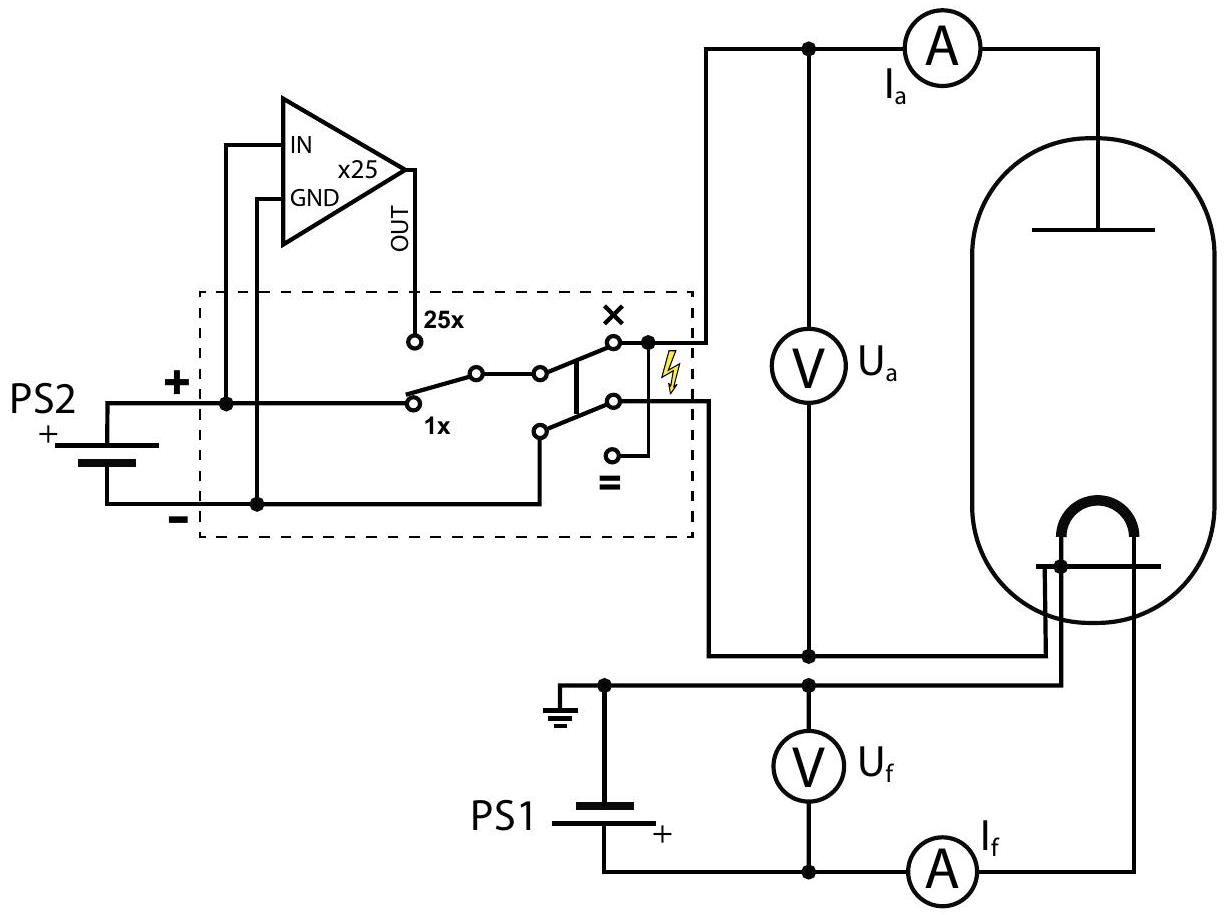
\includegraphics[width=0.6\linewidth]{zapojeni}
			\caption{Schéma zapojení}
			\label{fig:zapojeni}
		\end{figure}
		
		\section{Měření}
		Před samotným měřením je třeba nalézt optimální hodnoty stabilizačního napětí $U_1$ a brzdného napětí $U_3$. Hledáme nastavení s co největšími rozdíly mezi lokálními maximy a minimy měřeného kolektorového napětí, aby bylo možné co nejlépe při analýze dat samotná maxima určit. Potenciálovou bariéru se snažíme udělat co největší, mj. i proto, že se při měření kolektorového napětí chceme pohybovat v rámci rozsahu měřícího přístroje. Příliš nízké brzdné napětí zároveň nedokáže efektivně zpomalit elektrony, které byly součástí nepružných srážek. Pro stabilizační napětí $U_1$ postupně napětí zvyšujeme a sledujeme získaná data. Jako optimální vyhodnocujeme hodnoty
		\begin{equation*}
			U_1 = 2.1 \,\mathrm{V} \quad U_3 = 9.1 \,\mathrm{V}.
		\end{equation*}
		Závislost měřeného kolektorového napětí na urychlujícím při těchto hodnotách lze pozorovat na obrázku 2.
		
		\begin{figure}[H]
			\centering
			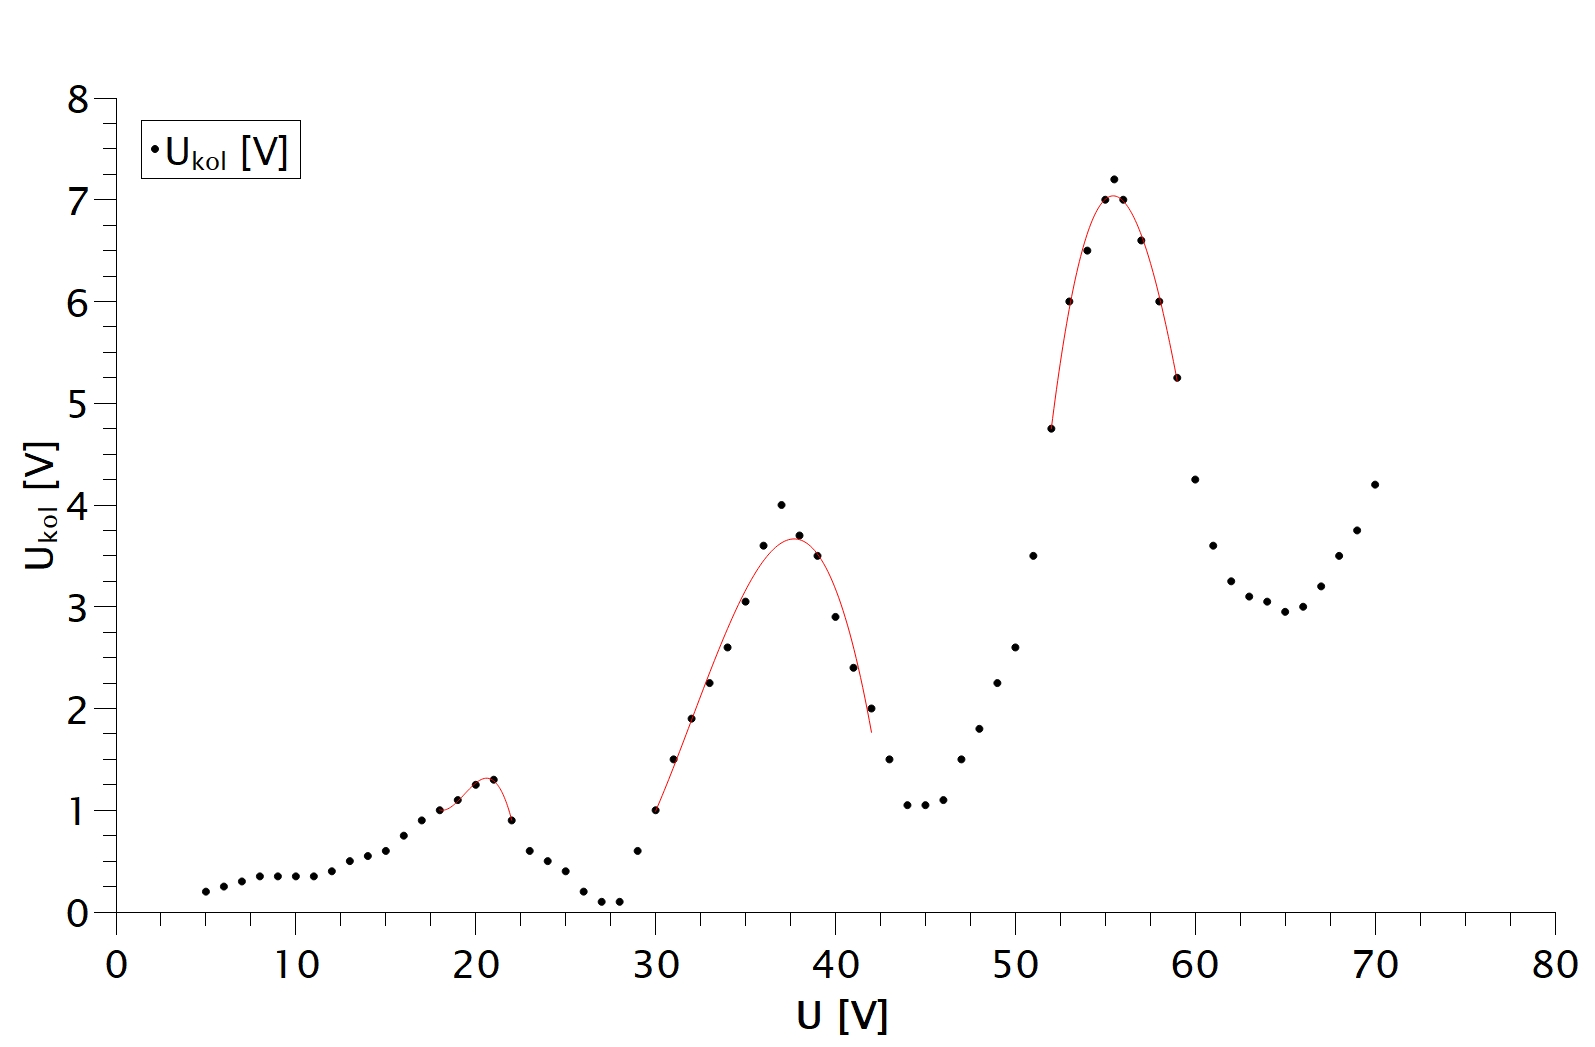
\includegraphics[width=0.9\linewidth]{mereni}
			\caption{Závislost kolektorového napětí na urychlujícím napětí}
			\label{fig:mereni}
		\end{figure}
		Z měření získáváme maxima při napětí:
		\begin{equation*}
			U_{max} = 20.61\pm 0.01, 37.70\pm0,01, 55.44 \pm 0.01\,\mathrm{V}
		\end{equation*}
		Z čehož získáváme hodnotu excitační energie:
		\begin{equation}
			E = 19.313 \pm 0.004 \,\rm eV,
		\end{equation}
		což je blízké excitační energii helia a neonu.\\
		Zároveň při spektrální analýze získáváme naprosto jasné emisní spektrum neonu, jak lze pozorovat na obrázku 3.
		\begin{figure}[H]
			\centering
			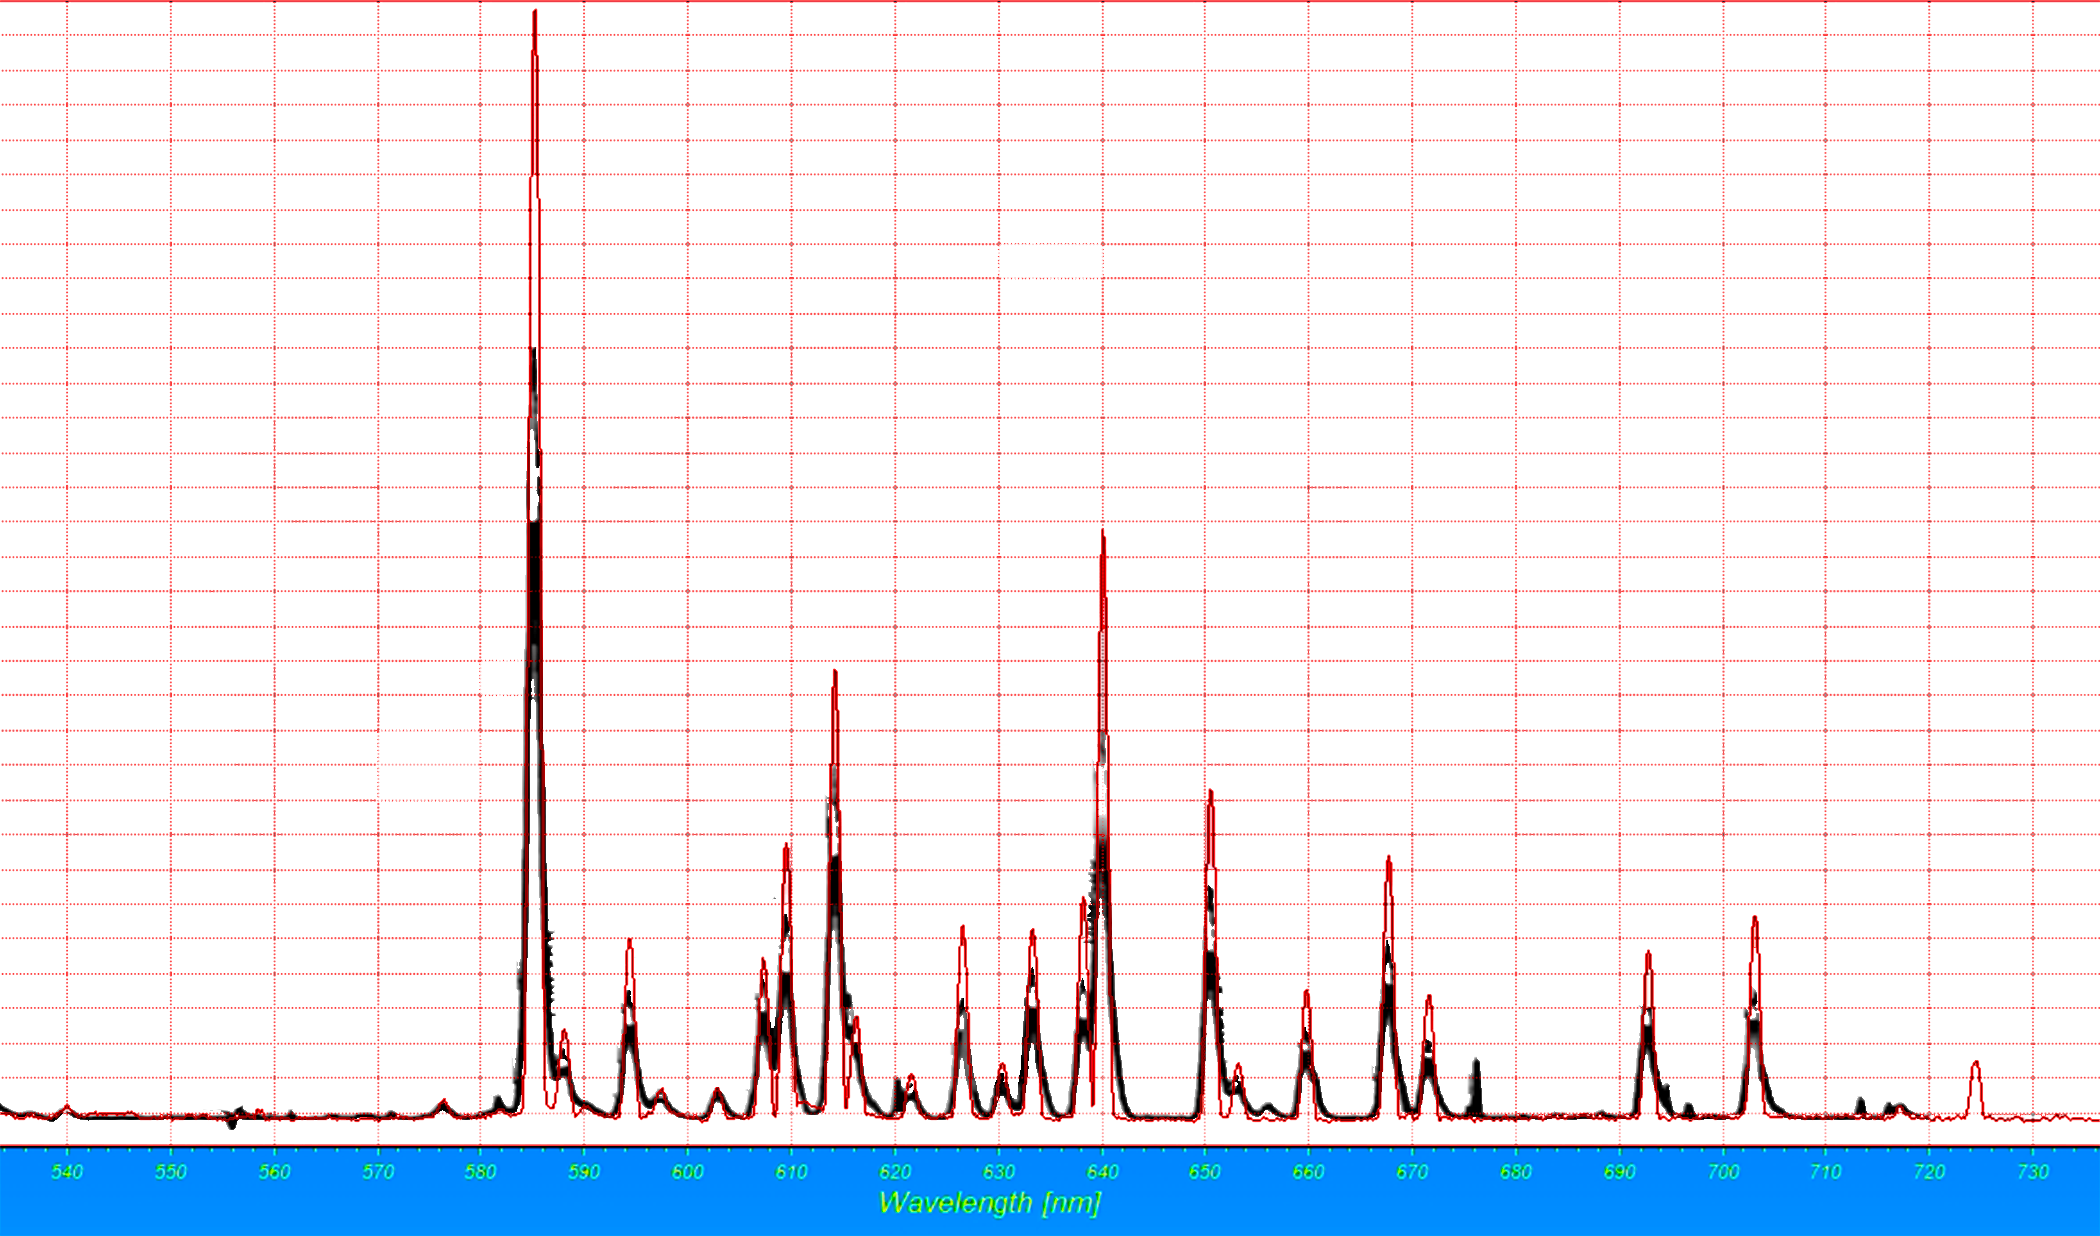
\includegraphics[width=1\linewidth]{spectrum3}
			\caption{naměřené emisní spektrum (červená) a spektrum neonu$^{[1]}$ (černá)}
		\end{figure}
		V trubici je tedy jistě neon, excitační energie však neodpovídá nejnižší energii pro neon, ta je totiž 16.6 eV$^{[2]}$.
		Tuto odchylku lze vysvětlit tím, že není realizován pouze nejnižší excitovaný stav, ale i stavy vyšší, jejichž energie se od prvního stavu liší o jednotky eV (obr. 5$^{[1]}$).
			\begin{figure}[H]
			\centering
			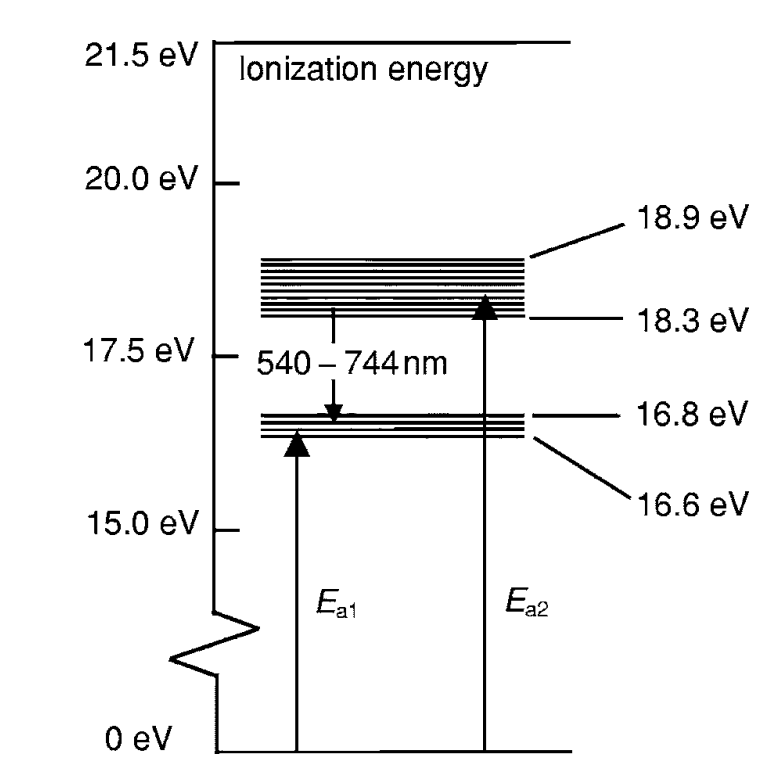
\includegraphics[width=0.8\linewidth]{hladiny}
			\caption{naměřené emisní spektrum}
		\end{figure}
		
		
		
		
		
		
		\section{Závěr}
		Podařilo se nám naměřit a zpracovat data pro určení excitační energie, spektrografickou analýzou se podařilo utvrdit, že plynem v trubici je neon. Následně jsme excitační energie s vysvětlením, že není realizována pouze nejnižší e. hladina, neonu přiřadili.
	
		

		
		\section{Zdroje}
		
		1. Usachev, A \& Zobnin, A \& Shonenkov, A \& Lipaev, A \& Molotkov, V \& Petrov, Oleg \& Fortov, Valdimir \& Pustylnik, M. \& Fink, M \& Thoma, M \& Thomas, Hubertus \& Padalka, G. (2018). Influence of dust particles on the neon spectral line intensities at the uniform positive column of dc discharge at the space apparatus “Plasma Kristall-4”. Journal of Physics: Conference Series. 946. \\ \\
		2.  Rapior, Gerald \& Sengstock, Klaus \& Baev, Valery. New features of the Franck-Hertz experiment. Am. J. Phys. 74, 423 American Association of Physics Teachers (AAPT), 2006.
		
	
		
		
		% Nakonec nezapomeňte projet text programem vlna nebo vlnka, např.
		% 	vlna -m -l -n mojeuloha.tex
		% nebo zkontrolovat a opravit jednopísmenné předložky na koncích řádků ručně.
	\end{multicols}
\end{document}
